\heading{数据结构与算法B-23春-期末}
\textbf{一、选择题（30 分，每小题 2 分）}

\begin{question}
下列叙述中正确的是（\quad）。
\begin{choiceoptions}[1]
  \item 散列是一种基于索引的逻辑结构
  \item 基于顺序表实现的逻辑结构属于线性结构
  \item 数据结构设计影响算法效率，逻辑结构起到了决定作用
  \item 一个逻辑结构可以有多种类型的存储结构，且不同类型的存储结构会直接影响到数据处理的效率
\end{choiceoptions}
\begin{solution}
选 D。逻辑结构描述数据元素之间的关系，存储结构描述这种关系在计算机中的实现方式。同一种逻辑结构可以采用顺序、链式、索引、散列等不同存储方式，不同存储方式会直接影响查找、插入、删除等操作效率。
\end{solution}
\end{question}

\begin{question}
在广度优先搜索算法中，一般使用什么辅助数据结构？（\quad）
\begin{choiceoptions}[2]
  \item 队列
  \item 栈
  \item 树
  \item 散列
\end{choiceoptions}
\begin{solution}
选 A。广度优先搜索按照“先发现的顶点先扩展”的顺序进行，符合队列的先进先出特性。
\end{solution}
\end{question}

\begin{question}
若某线性表实现采取链式存储，那么该线性表中结点的存储地址（\quad）。
\begin{choiceoptions}[2]
  \item 一定不连续
  \item 既可连续亦可不连续
  \item 一定连续
  \item 与头结点存储地址保持连续
\end{choiceoptions}
\begin{solution}
选 B。链式存储通过引用或链接表示结点之间的逻辑关系，结点的物理地址不要求连续；实际分配时也可能碰巧连续，因此应表述为既可连续也可不连续。
\end{solution}
\end{question}

\begin{question}
若某线性表的常用操作是在表尾插入或删除元素，则时间开销最小的存储方式是（\quad）。
\begin{choiceoptions}[1]
  \item 单链表
  \item 仅有头引用的单循环链表
  \item 顺序表
  \item 仅有尾引用的单循环链表
\end{choiceoptions}
\begin{solution}
选 C。顺序表在表尾插入、删除元素通常只需修改表长，时间为 $O(1)$（不考虑扩容）。单链表或单循环链表若要删除尾结点，通常需要寻找尾结点前驱，时间为 $O(n)$。
\end{solution}
\end{question}

\begin{question}
给定后缀表达式（逆波兰式）\texttt{ab+-c*d-}，其对应的中缀表达式是（\quad）。
\begin{choiceoptions}[1]
  \item \texttt{a-b-c*d}
  \item \texttt{-(a+b)*c-d}
  \item \texttt{a+b*c-d}
  \item \texttt{(a+b)*(-c-d)}
\end{choiceoptions}
\begin{solution}
选 B。先由 \texttt{ab+} 得到 $(a+b)$，随后的一元负号得到 $-(a+b)$；再与 $c$ 相乘，最后减去 $d$，即 $-(a+b)c-d$。
\end{solution}
\end{question}

\begin{question}
今有一空栈 $S$，基于待进栈的数据元素序列 $a,b,c,d,e,f$，依次进行进栈、进栈、出栈、进栈、进栈、出栈的一系列操作，上述操作完成以后，栈 $S$ 的栈顶元素为（\quad）。
\begin{choiceoptions}[4]
  \item $f$
  \item $c$
  \item $a$
  \item $b$
\end{choiceoptions}
\begin{solution}
选 B。操作过程为：$a$ 入栈、$b$ 入栈、弹出 $b$、$c$ 入栈、$d$ 入栈、弹出 $d$，此时栈中自底向顶为 $a,c$，栈顶为 $c$。
\end{solution}
\end{question}

\begin{question}
对于带头结点的单链表，其表头为 \texttt{head}，则判定空表的条件是（\quad）。
\begin{choiceoptions}[2]
  \item \texttt{head is None}
  \item \texttt{head is not None}
  \item \texttt{head.next is head}
  \item \texttt{head.next is None}
\end{choiceoptions}
\begin{solution}
选 D。带头结点的单链表即使为空也保留头结点；在 Python 风格的链表表示中，空表时头结点的 \texttt{next} 引用为空，因此条件为 \texttt{head.next is None}。
\end{solution}
\end{question}

\begin{question}
以下典型排序算法中，具有稳定排序特性的是（\quad）。
\begin{choiceoptions}[1]
  \item 冒泡排序（Bubble Sort）
  \item 直接选择排序（Selection Sort）
  \item 快速排序（Quick Sort）
  \item 希尔排序（Shell Sort）
\end{choiceoptions}
\begin{solution}
选 A。冒泡排序只交换逆序的相邻元素，相等元素通常不会交换，所以稳定；直接选择排序、快速排序和希尔排序一般都不稳定。
\end{solution}
\end{question}

\begin{question}
以下关键字序列中，可以有效构成一个大根堆（即最大值堆，最大值在堆顶）的序列是（\quad）。
\begin{choiceoptions}[1]
  \item $5,8,1,3,9,6,2,7$
  \item $9,8,1,7,5,6,2,3$
  \item $9,8,6,3,5,1,2,7$
  \item $9,8,6,7,5,1,2,3$
\end{choiceoptions}
\begin{solution}
选 D。按顺序存储的堆满足每个父结点关键字都不小于其左右孩子。D 中 $9\ge 8,6$，$8\ge 7,5$，$6\ge 1,2$，$7\ge 3$，满足大根堆性质。
\end{solution}
\end{question}

\begin{question}
以下典型排序算法中，内存开销最大的是（\quad）。
\begin{choiceoptions}[2]
  \item 冒泡排序
  \item 快速排序
  \item 归并排序
  \item 堆排序
\end{choiceoptions}
\begin{solution}
选 C。归并排序通常需要 $O(n)$ 的辅助数组；快速排序主要使用递归栈，平均 $O(\log n)$；冒泡排序和堆排序通常为 $O(1)$ 额外空间。
\end{solution}
\end{question}

\begin{question}
排序算法往往依赖于对待排序元素序列的多趟比较/移动操作（即执行多轮循环），第一趟结束后，任一元素都无法确定其最终排序位置的算法是（\quad）。
\begin{choiceoptions}[2]
  \item 选择排序
  \item 快速排序
  \item 冒泡排序
  \item 插入排序
\end{choiceoptions}
\begin{solution}
选 D。选择排序第一趟可确定最小（或最大）元素的位置；快速排序一趟划分后枢轴到达最终位置；冒泡排序第一趟通常可确定一个最大（或最小）元素的位置。插入排序第一趟只保证局部有序，元素最终位置不能确定。
\end{solution}
\end{question}

\begin{question}
考察以下基于单链表的操作，相较于顺序表实现，带来更高时间复杂度的操作是（\quad）。
\begin{choiceoptions}[1]
  \item 合并两个有序线性表，并保持合成后的线性表依然有序
  \item 交换第一个元素与第二个元素的值
  \item 查找某一元素值是否在线性表中出现
  \item 输出第 $i$ 个（$0\le i<n$，$n$ 为元素个数）元素
\end{choiceoptions}
\begin{solution}
选 D。顺序表可按下标随机访问，第 $i$ 个元素访问为 $O(1)$；单链表必须从头引用开始逐结点后移，访问第 $i$ 个元素为 $O(i)$，时间复杂度更高。
\end{solution}
\end{question}

\begin{question}
已知一个整型数组中的元素值依次为 $\{19,20,50,61,73,85,11,39\}$，采用某种排序算法，在多趟比较/移动操作后，依次得到如下中间结果：
\[
\begin{array}{l}
(1)\ 19\ 20\ 11\ 39\ 73\ 85\ 50\ 61,\\
(2)\ 11\ 20\ 19\ 39\ 50\ 61\ 73\ 85,\\
(3)\ 11\ 19\ 20\ 39\ 50\ 61\ 73\ 85.
\end{array}
\]
请问，上述过程使用的排序算法是（\quad）算法。
\begin{choiceoptions}[4]
  \item 冒泡排序
  \item 插入排序
  \item 希尔排序
  \item 归并排序
\end{choiceoptions}
\begin{solution}
选 C。第一趟结果类似按增量 $4$ 分组排序：$(19,73)$、$(20,85)$、$(50,11)$、$(61,39)$ 分别调整后得到 $19,20,11,39,73,85,50,61$；之后增量减小继续排序，符合希尔排序过程。
\end{solution}
\end{question}

\begin{question}
今有一非连通无向图，共有 $36$ 条边，该图至少有（\quad）个顶点。
\begin{choiceoptions}[4]
  \item $8$
  \item $9$
  \item $10$
  \item $11$
\end{choiceoptions}
\begin{solution}
选 C。若 $n$ 个顶点的无向图非连通，则边数最多时可由 $n-1$ 个顶点组成完全图，另一个顶点孤立，最多边数为 $\binom{n-1}{2}$。令 $\binom{n-1}{2}\ge 36$，最小满足的是 $n-1=9$，故 $n=10$。
\end{solution}
\end{question}

\begin{question}
令 $G=(V,E)$ 是一个无向图，若 $G$ 中任何两个顶点之间均存在唯一的简单路径相连，则下面说法中错误的是（\quad）。
\begin{choiceoptions}[1]
  \item 图 $G$ 中添加任何一条边，不一定造成图包含一个环
  \item 图 $G$ 中移除任意一条边得到的图均不连通
  \item 图 $G$ 的逻辑结构实际上退化为树结构
  \item 图 $G$ 中边的数目一定等于顶点数目减 $1$
\end{choiceoptions}
\begin{solution}
选 A。任意两点之间存在唯一简单路径说明 $G$ 是一棵树。树中任意两个顶点之间已有一条唯一简单路径，再添加一条边会和原路径构成一个环，因此 A 错误；B、C、D 都是树的性质。
\end{solution}
\end{question}

\textbf{二、判断题（10 分，每小题 1 分；对填写 Y，错填写 N）}

\begin{question}
按照前序、中序、后序方式周游一棵二叉树，分别得到不同的结点周游序列，然而三种不同的周游序列中，叶子结点都将以相同的顺序出现。（\quad）
\begin{solution}
答案：Y。无论采用前序、中序还是后序遍历，叶子结点之间的相对次序都与它们在树中的从左到右次序一致，因此叶子结点在三种序列中的相对顺序相同。
\end{solution}
\end{question}

\begin{question}
构建一个含 $N$ 个结点的（二叉）最小值堆，时间效率最优情况下的时间复杂度大 $O$ 表示为 $O(N\log N)$。（\quad）
\begin{solution}
答案：N。若采用自底向上的建堆方法，建堆时间复杂度为 $O(N)$，优于逐个插入造成的 $O(N\log N)$。
\end{solution}
\end{question}

\begin{question}
对任意一个连通的无向图，如果存在一个环，且这个环中的某一条边的权值不小于该环中任意一个其它的边的权值，那么这条边一定不会是该无向图的最小生成树中的边。（\quad）
\begin{solution}
答案：N。环性质要求“严格大于”环中其它边的边一定不在任何最小生成树中；若只是“不小于”，可能与其它边权值相等，此时该边仍可能出现在某棵最小生成树中。
\end{solution}
\end{question}

\begin{question}
通过树的周游可以求得树的高度，若采取深度优先遍历方式设计求解树高度问题的算法，算法空间复杂度大 $O$ 表示为 $O(\text{树的高度})$。（\quad）
\begin{solution}
答案：Y。深度优先遍历递归求树高时，递归栈深度等于当前根到结点的路径长度，最大为树高，因此辅助空间为 $O(h)$。
\end{solution}
\end{question}

\begin{question}
树可以等价转化二叉树，树的先序遍历序列与其相应的二叉树的前序遍历序列相同。（\quad）
\begin{solution}
答案：Y。树转化为二叉树通常采用“左孩子右兄弟”表示，树的先根遍历与转换后二叉树的先序遍历访问顺序一致。
\end{solution}
\end{question}

\begin{question}
如果一个连通无向图 $G$ 中所有边的权值均不同，则 $G$ 具有唯一的最小生成树。（\quad）
\begin{solution}
答案：Y。边权互异时，Kruskal 或 Prim 每一步对最小安全边的选择不会出现并列，从而最小生成树唯一。
\end{solution}
\end{question}

\begin{question}
求解最小生成树问题时，Kruskal 算法更适用于稀疏图，Prim 算法更适用于稠密图。（\quad）
\begin{solution}
答案：Y。Kruskal 主要按边排序和并查集合并，适合边数较少的稀疏图；Prim 使用邻接矩阵时可在 $O(n^2)$ 内完成，常用于稠密图。
\end{solution}
\end{question}

\begin{question}
使用线性探测法处理散列表碰撞问题，若表中仍有空槽（空单元），插入操作一定成功。（\quad）
\begin{solution}
答案：Y。线性探测按固定步长 $1$ 循环检查表中位置，只要探测过程完整且散列表仍有空槽，最终一定能找到空槽插入。
\end{solution}
\end{question}

\begin{question}
从链表中删除某个指定值的结点，其时间复杂度是 $O(1)$。（\quad）
\begin{solution}
答案：N。若只给定要删除的值，必须先从链表中查找该值所在结点及其前驱，查找过程平均和最坏都可能为 $O(n)$。
\end{solution}
\end{question}

\begin{question}
弗洛伊德（Floyd）算法是一种求解有向和无向图最短路径的动态规划算法，但该算法的局限性是无法正确求解带有负权值边的图的最短路径。（\quad）
\begin{solution}
答案：N。Floyd 算法可以处理负权边，但不能处理存在可达负权回路的情形；只要不存在负权回路，负权边并不妨碍正确求解最短路径。
\end{solution}
\end{question}

\textbf{三、填空题（20 分，每题 2 分）}

\begin{question}
定义二叉树中一个结点的度数为其子结点的个数。现有一棵结点总数为 $101$ 的二叉树，其中度数为 $1$ 的结点有 $30$ 个，则度数为 $0$ 结点有 \blank 个。
\begin{solution}
答案：$36$。设度为 $0,1,2$ 的结点数分别为 $n_0,n_1,n_2$。二叉树有性质 $n_0=n_2+1$，且 $n_0+n_1+n_2=101$，已知 $n_1=30$，所以 $n_0+n_2=71$，解得 $n_2=35,n_0=36$。
\end{solution}
\end{question}

\begin{question}
定义完全二叉树的根结点所在层为第一层，如果一个二叉树的第六层有 $23$ 个叶结点，则它的总结点数量可能有 \blank 个。（请填写所有 $3$ 个可能的结点数。）
\begin{solution}
答案：$54,80,81$。若树高为 $6$，前 $5$ 层共有 $2^5-1=31$ 个结点，第六层有 $23$ 个叶结点，总数为 $31+23=54$。若树高为 $7$，第六层满 $32$ 个结点，其中有孩子的第六层结点数为 $32-23=9$；第七层结点数可为 $17$ 或 $18$，总数为 $31+32+17=80$ 或 $31+32+18=81$。
\end{solution}
\end{question}

\begin{question}
对于初始排序码序列 $(51,41,31,21,61,71,81,11,91)$，第 $1$ 趟快速排序（以第一个数字为 pivot 轴值）的结果是：\blank。
\begin{solution}
答案：$(11,41,31,21,51,71,81,61,91)$。以 $51$ 为枢轴，从右向左找到小于 $51$ 的 $11$ 放到左端空位，再从左向右找到大于 $51$ 的 $61$ 放到右端空位，最后左右下标相遇，将 $51$ 放入中间位置，得到该划分结果。
\end{solution}
\end{question}

\begin{question}
如果输入序列是已经正序，在（改进）冒泡排序、直接插入排序和直接选择排序算法中，\blank 算法最慢结束。
\begin{solution}
答案：直接选择排序。改进冒泡排序在一趟扫描无交换后即可结束，为 $O(n)$；直接插入排序对正序序列也近似 $O(n)$；直接选择排序无论初始序列如何都要进行多轮选择比较，仍为 $O(n^2)$。
\end{solution}
\end{question}

\begin{question}
已知某二叉树的先根周游序列为 $\{A,B,D,E,C,F,G\}$，中根周游序列为 $\{D,B,E,A,C,G,F\}$，则该二叉树的后根次序周游序列为 $\{\blank\}$。
\begin{solution}
答案：$D,E,B,G,F,C,A$。先序首元素 $A$ 为根，中序以 $A$ 分成左子树 $D,B,E$ 和右子树 $C,G,F$。左子树根为 $B$，后序为 $D,E,B$；右子树根为 $C$，其右子树根为 $F$ 且 $G$ 为 $F$ 的左孩子，后序为 $G,F,C$；合并得 $D,E,B,G,F,C,A$。
\end{solution}
\end{question}

\begin{question}
使用栈计算后缀表达式（操作数均为一位数）\texttt{1 2 3 + 4 * 5 + 3 + -}，当扫描到第二个 \texttt{+} 号但还未对该 \texttt{+} 号进行运算时，栈的内容（以栈底到栈顶从左往右的顺序书写）为 \blank。
\begin{solution}
答案：$1,20,5$。扫描 $1,2,3,+$ 后，$2+3=5$，栈为 $1,5$；再扫描 $4,*$ 后，$5\times4=20$，栈为 $1,20$；继续扫描操作数 $5$ 后遇到第二个加号，尚未计算前栈为 $1,20,5$。
\end{solution}
\end{question}

\begin{question}
$51$ 个顶点的连通图 $G$ 有 $50$ 条边，其中权值为 $1,2,3,4,5,6,7,8,9,10$ 的边各 $5$ 条，则连通图 $G$ 的最小生成树各边的权值之和为 \blank。
\begin{solution}
答案：$275$。$51$ 个顶点的连通图若只有 $50$ 条边，则它本身就是一棵树；树的最小生成树就是自身。因此权值和为 $5(1+2+\cdots+10)=5\times55=275$。
\end{solution}
\end{question}

\begin{question}
包含 $n$ 个顶点无向图的邻接表存储结构中，所有顶点的边表中最多有 \blank 个结点。具有 $n$ 个顶点的有向图，一个顶点入度和出度之和最大值不超过 \blank。
\begin{solution}
答案：$n(n-1)$；$2(n-1)$。无向简单图最多有 $\binom{n}{2}$ 条边，邻接表中每条无向边出现两次，因此最多有 $n(n-1)$ 个边表结点。有向图中一个顶点最多向其它 $n-1$ 个顶点发出边，也最多从其它 $n-1$ 个顶点接收边，所以入度与出度之和最大为 $2(n-1)$。
\end{solution}
\end{question}

\begin{question}
给定一个长度为 $7$ 的空散列表，采用双散列法解决冲突，两个散列函数分别为 $h_1(key)=key\%7$，$h_2(key)=key\%5+1$。请向散列表依次插入关键字为 $30,58,65$ 的集合元素，插入完成后 $65$ 在散列表中存储地址为 \blank。
\begin{solution}
答案：$3$。$30\%7=2$，先放入地址 $2$；$58\%7=2$ 发生冲突，步长 $58\%5+1=4$，放入 $(2+4)\%7=6$；$65\%7=2$ 也冲突，步长 $65\%5+1=1$，下一地址为 $3$，故 $65$ 存在地址 $3$。
\end{solution}
\end{question}


\begin{question}
阅读 Python 算法 \texttt{ABC}，回答问题。
\begin{pycode}
from math import isqrt

def ABC(n):
    m = isqrt(n)
    for k in range(2, m + 1):
        if n % k == 0:
            return 0
    return 1
\end{pycode}
(1) 算法的功能是：\blank。\par
(2) 算法的时间复杂度是 $O($\blank$)$。
\begin{solution}
答案：(1) 判断 $n$ 是否为素数（若没有 $2$ 到 $\lfloor\sqrt n\rfloor$ 范围内的因子则返回 $1$，否则返回 $0$）；(2) $\sqrt n$。Python 中 \texttt{isqrt(n)} 返回 $\lfloor\sqrt n\rfloor$，循环最多检查从 $2$ 到 $\lfloor\sqrt n\rfloor$ 的整数因子，因此时间复杂度为 $O(\sqrt n)$。
\end{solution}
\end{question}

\textbf{四、简答题（3 题，共 14 分）}

\begin{question}[字符串匹配与 KMP]
字符串匹配算法从长度为 $n$ 的文本串 $S$ 中查找长度为 $m$ 的模式串 $P$ 的首次出现位置。
\begin{enumerate}
  \item 字符串匹配的朴素算法使用暴力搜索，大致过程如下：对于 $P$ 在 $S$ 中可能出现的 $n-m+1$ 个位置，比对此位置时 $P$ 和 $S$ 中对应子串是否相等。其时间复杂度 $O((n-m+1)m)$。请举例说明算法时间复杂度一种最坏情况（注：例子中请只出现 $0$ 和 $1$ 两种字符）。
  \item 已知字符串 $S$ 为 \texttt{abaabaabacacaabaabcc}，模式串 $t$ 为 \texttt{abaabc}。采用 KMP 算法进行查找，请写出 \texttt{next} 数组。
  \item 说明在上述 (2) 步骤中，第一次出现不匹配（\texttt{s[i] != t[j]}）时，$i=j=5$；则下次比对时，$i$ 和 $j$ 的值分别是？
\end{enumerate}
\begin{solution}
(1) 可取文本串 $S=00\cdots 00$，模式串 $P=00\cdots 01$（前 $m-1$ 位为 $0$，最后一位为 $1$）。每个可能起始位置都会先匹配很多个 $0$，最后才因 $1$ 不匹配而失败，从而达到 $O((n-m+1)m)$ 的最坏量级。\par
(2) 采用下标从 $0$ 开始且 \texttt{next[0] = -1} 的常见定义，$t=\texttt{abaabc}$ 的 \texttt{next} 数组为
\[
[-1,0,0,1,1,2].
\]
(3) 第一次不匹配在 $i=j=5$，失配后 $i$ 不回退，$j$ 回退到 \texttt{next[5]}，所以下次比对时 $i=5,j=2$。
\end{solution}
\end{question}

\begin{question}[AOV 网络与拓扑排序]
有八项活动，每项活动标记为 $V_n(0\le n\le 7)$，每项活动要求的前驱如下：
\[
\begin{array}{c|cccccccc}
\text{活动} & V0 & V1 & V2 & V3 & V4 & V5 & V6 & V7 \\ \hline
\text{前驱} & \text{无前驱} & V0 & V0 & V0,V2 & V1 & V2,V4 & V3 & V5,V6
\end{array}
\]
试画出相应的 AOV 网络，并给出一个拓扑排序序列，如存在多种，则按照编号从小到大排序，输出最小的一种。
\begin{solution}
由前驱关系得到边：$V0\to V1,V2,V3$，$V1\to V4$，$V2\to V3,V5$，$V4\to V5$，$V3\to V6$，$V5\to V7$，$V6\to V7$。一个可画作如下的 AOV 网络：
\begin{center}
\begin{tikzpicture}[>=stealth, node distance=1.8cm, every node/.style={draw,circle,minimum size=7mm,inner sep=1pt}]
  \node (v0) {$V0$};
  \node[right=of v0, yshift=1.1cm] (v1) {$V1$};
  \node[right=of v0, yshift=-0.1cm] (v2) {$V2$};
  \node[right=of v2, yshift=-1.0cm] (v3) {$V3$};
  \node[right=of v1] (v4) {$V4$};
  \node[right=of v4, yshift=-0.9cm] (v5) {$V5$};
  \node[right=of v3] (v6) {$V6$};
  \node[right=of v5, yshift=-0.4cm] (v7) {$V7$};
  \draw[->] (v0) -- (v1);
  \draw[->] (v0) -- (v2);
  \draw[->] (v0) -- (v3);
  \draw[->] (v1) -- (v4);
  \draw[->] (v2) -- (v3);
  \draw[->] (v2) -- (v5);
  \draw[->] (v4) -- (v5);
  \draw[->] (v3) -- (v6);
  \draw[->] (v5) -- (v7);
  \draw[->] (v6) -- (v7);
\end{tikzpicture}
\end{center}
每次在当前入度为 $0$ 的顶点中选编号最小者，得到拓扑序列
\[
V0,V1,V2,V3,V4,V5,V6,V7.
\]
\end{solution}
\end{question}

\begin{question}[Huffman 树与 Huffman 编码]
简要回答下列 Huffman 树以及 Huffman 编码的相关问题。
\begin{enumerate}
  \item 假定需要编码的字符个数为 $m$，哈夫曼树构造后结点总数多少？简要阐述理由。
  \item 假定报文中各字符及其出现次数为：$A(50),B(30),C(10),D(25),E(11),F(99),G(8),H(51),I(22)$。试画出对应的 Huffman 树（严格按照左小右大构造），并给出各个字符的 Huffman 编码（左分支编码 $0$，右分支编码 $1$）。
\end{enumerate}
\begin{solution}
(1) 结点总数为 $2m-1$。Huffman 树是具有 $m$ 个叶子结点的满二叉树，每次合并两个结点产生一个新内部结点，总共合并 $m-1$ 次，因此内部结点数为 $m-1$，总结点数为 $m+(m-1)=2m-1$。\par
(2) 按权值从小到大反复合并，过程为：$8+10=18$，$11+18=29$，$22+25=47$，$29+30=59$，$47+50=97$，$51+59=110$，$97+99=196$，$110+196=306$。严格左小右大时，编码为：
\[
\begin{array}{c|ccccccccc}
\text{字符} & A&B&C&D&E&F&G&H&I \\ \hline
\text{编码} & 101&011&01011&1001&0100&11&01010&00&1000
\end{array}
\]
对应树可表示为：
\begin{center}
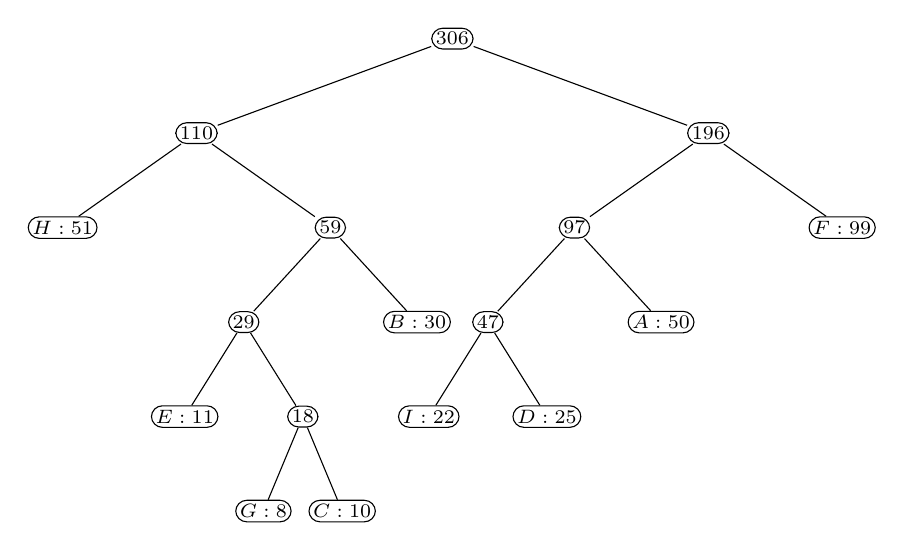
\begin{tikzpicture}[
  level distance=12mm,
  level 1/.style={sibling distance=65mm},
  level 2/.style={sibling distance=34mm},
  level 3/.style={sibling distance=22mm},
  level 4/.style={sibling distance=15mm},
  level 5/.style={sibling distance=10mm},
  every node/.style={draw,rounded corners,align=center,inner sep=1.5pt,font=\scriptsize}
]
\node {306}
  child {node {110}
    child {node {$H:51$}}
    child {node {59}
      child {node {29}
        child {node {$E:11$}}
        child {node {18}
          child {node {$G:8$}}
          child {node {$C:10$}}
        }
      }
      child {node {$B:30$}}
    }
  }
  child {node {196}
    child {node {97}
      child {node {47}
        child {node {$I:22$}}
        child {node {$D:25$}}
      }
      child {node {$A:50$}}
    }
    child {node {$F:99$}}
  };
\end{tikzpicture}
\end{center}
\end{solution}
\end{question}

\textbf{五、算法填空（4 题，共 26 分）}


\begin{question}[有序链表删除重复元素]
请填空完成下列 Python 程序：读入一个从小到大排好序的整数序列到链表，然后在链表中删除重复的元素，使得重复的元素只保留 $1$ 个，然后将整个链表内容输出。

输入：第一行是正整数 $n(n<80)$，第二行是 $n$ 个整数。输入样例为 $9$ 和 \texttt{1 2 2 2 3 3 4 4 6}，输出样例为 \texttt{1 2 3 4 6}。
\begin{pycode}
class Node:
    def __init__(self, data):
        self.data = data
        self.next = None

n = int(input())
a = list(map(int, input().split()))
head = Node(a[0])
p = head
for x in a[1:]:
    p.next = Node(__________)                  # (1)
    p = __________                             # (2)

p = head
while p is not None:
    while __________ and p.data == p.next.data: # (3)
        __________                              # (4)
    p = p.next

p = head
while p is not None:
    print(p.data, end=" ")
    __________                                  # (5)
\end{pycode}
\begin{solution}
空白处依次为：
\begin{enumerate}
  \item \texttt{x}
  \item \texttt{p.next}
  \item \texttt{p.next is not None}
  \item \texttt{p.next = p.next.next}
  \item \texttt{p = p.next}
\end{enumerate}
建链时，\texttt{p.next} 是新建结点，随后令 \texttt{p} 后移到这个新结点。删除重复值时，由于序列已有序，重复元素必相邻；只要 \texttt{p.next} 存在且数据相等，就让 \texttt{p.next} 越过重复结点。输出时每打印一个结点后将 \texttt{p} 后移。
\end{solution}
\end{question}


\begin{question}[堆排序]
为实现对一组数据根据排序码进行自小到大排序，请填空完成下列 Python 堆排序程序（仅含关键部分代码）。每条记录用字典表示，其中 \texttt{record["key"]} 为排序码。程序中建立的堆是大根堆（即最大值堆，最大元素在堆顶）。
\begin{pycode}
def sift(records, i, n):
    temp = records[i]
    child = __________                         # (1)
    while child < n:
        if __________ and records[child]["key"] < records[child + 1]["key"]: # (2)
            child += 1
        if temp["key"] < records[child]["key"]:
            __________                         # (3)
            i = child
            child = __________                 # (4)
        else:
            break
    records[i] = temp


def heap_sort(records):
    n = len(records)
    for i in range(n // 2 - 1, -1, -1):
        __________                             # (5)
    for i in range(n - 1, 0, -1):
        records[0], records[i] = records[i], records[0]
        __________                             # (6)
\end{pycode}
\begin{solution}
空白处依次为：
\begin{enumerate}
  \item \texttt{2 * i + 1}
  \item \texttt{child < n - 1}
  \item \texttt{records[i] = records[child]}
  \item \texttt{2 * i + 1}
  \item \texttt{sift(records, i, n)}
  \item \texttt{sift(records, 0, i)}
\end{enumerate}
在 $0$ 下标存储的完全二叉树中，结点 $i$ 的左孩子为 $2i+1$，右孩子为 $2i+2$。调整大根堆时应先选择较大的孩子，再将较大孩子上移。每次把堆顶最大元素交换到末尾后，只需对剩余区间 $[0,i)$ 再调整堆。Python 的 \texttt{range(n // 2 - 1, -1, -1)} 会从最后一个非叶结点一直枚举到根结点 $0$。
\end{solution}
\end{question}


\begin{question}[AOV 网的拓扑排序程序]
以下 Python 代码实现了对 AOV 网的拓扑排序。设 \texttt{graph[i]} 存放从顶点 $i$ 出发的所有邻接点编号，请阅读代码并补全空缺。
\begin{pycode}
def find_indegree(graph):
    indegree = [0] * len(graph)
    for i in range(len(graph)):
        for v in graph[i]:
            __________                         # (1)
    return indegree


def topo_sort(graph):
    indegree = find_indegree(graph)
    stack = []
    topo = []
    for i in range(len(graph)):
        if indegree[i] == 0:
            __________                         # (2)

    while __________:                          # (3)
        j = stack.pop()
        topo.append(j)
        for k in __________:                   # (4)
            indegree[k] = __________           # (5)
            if indegree[k] == 0:
                __________                     # (6)

    if __________:                             # (7)
        print("The aov network has a cycle")
        return None
    return topo
\end{pycode}
\begin{solution}
空白处依次为：
\begin{enumerate}
  \item \texttt{indegree[v] += 1}
  \item \texttt{stack.append(i)}
  \item \texttt{stack}
  \item \texttt{graph[j]}
  \item \texttt{indegree[k] - 1}
  \item \texttt{stack.append(k)}
  \item \texttt{len(topo) < len(graph)}
\end{enumerate}
求入度时，每扫描到一条指向顶点 \texttt{v} 的边，就将该顶点入度加一。拓扑排序过程中，栈中保存当前入度为 $0$ 的顶点；弹出一个顶点并输出后，需要把它所有后继顶点的入度减 $1$。若最终输出顶点数小于图中顶点数，说明仍有顶点未输出，AOV 网中存在环。
\end{solution}
\end{question}


\begin{question}[无向图连通性与回路判断]
请填空完成下列 Python 程序：给定一个无向图，判断是否连通，是否有回路。图用邻接矩阵 \texttt{G} 表示，\texttt{G[v][u] == 1} 表示顶点 $v$ 与顶点 $u$ 相邻。
\begin{pycode}
def dfs_connection(G, visited, v):
    visited[v] = True
    total = 1
    for u in range(len(G)):
        if G[v][u] and not visited[u]:
            total += dfs_connection(G, visited, u)
    return total


def dfs_loop(G, visited, v, parent):
    visited[v] = True
    for u in range(len(G)):
        if G[v][u]:
            if not visited[u]:
                if __________:                 # (1)
                    return True
            else:
                if __________:                 # (2)
                    return True
    return False

n, m = map(int, input().split())
G = [[0] * n for _ in range(n)]
for _ in range(m):
    a, b = map(int, input().split())
    G[a][b] = G[b][a] = 1

visited = [False] * n
total = dfs_connection(G, visited, 0)
if __________:                                 # (3)
    print("connected:yes")
else:
    print("connected:no")

visited = [False] * n
loop_found = False
for i in range(n):
    if __________:                             # (4)
        if dfs_loop(G, visited, i, -1):
            loop_found = True
            break

if loop_found:
    print("loop:yes")
else:
    print("loop:no")
\end{pycode}
\begin{solution}
空白处依次为：
\begin{enumerate}
  \item \texttt{dfs\_loop(G, visited, u, v)}
  \item \texttt{u != parent}
  \item \texttt{total == n}
  \item \texttt{not visited[i]}
\end{enumerate}
第一次 DFS 后，若访问到的顶点总数等于 $n$，图连通。判断无向图是否有环时，从 $v$ 访问到未访问的邻接点 $u$ 就递归；若邻接点已经访问过且不是 DFS 树上 $v$ 的父结点 \texttt{parent}，则发现回边，说明存在回路。外层循环能处理非连通图的每个连通分量。
\end{solution}
\end{question}
